% ============================================================
%  midsub_v3.tex -- EVS Project #19 Mid-Evaluation (version 3: concise)
%  Same topics as midsub_v2.tex, much less text.
%  Compile (from slides/): pdflatex midsub_v3; bibtex midsub_v3;
%                          pdflatex midsub_v3; pdflatex midsub_v3
%  Numbers: same sources as midsub.tex / midsub_v2.tex (see NUMBERS.md).
% ============================================================
\documentclass[11pt,aspectratio=169]{beamer}

\usetheme{Madrid}
\usecolortheme{seahorse}

\usepackage[T1]{fontenc}
\usepackage[utf8]{inputenc}
\usepackage{tikz}
\usetikzlibrary{positioning, arrows.meta}
\usepackage{booktabs}
\usepackage{graphicx}
\usepackage{multirow}
\usepackage{array}
\newcolumntype{L}[1]{>{\raggedright\arraybackslash}p{#1}}
\usepackage{natbib}
\bibliographystyle{unsrtnat}

\newcommand{\FigPath}[1]{../figures/#1.png}
\newcommand{\Fig}[2]{\includegraphics[width=#2,height=0.66\textheight,keepaspectratio]{\FigPath{#1}}}

\title[Compound Heat-Drought Stress]{Compound Heat--Drought Stress over India}
\subtitle{Are ecosystems hit harder when heat and drought strike together?\\[2pt]
  \small Mid-Evaluation, EVS Project \#19}
\author[Deshmukh et al.]{
  Arnav Deshmukh \and Ayush Brajesh Roy \and Saksham Chitkara \and
  Gracy Garg \and Rudra Choudhary
}
\institute{IIIT Hyderabad}
\date{\today}

\begin{document}

\frame{\titlepage}

\begin{frame}{Outline}
  \tableofcontents
\end{frame}

% =================================================================
\section{Problem statement \& motivation}
% =================================================================

\begin{frame}{Heat and drought rarely come alone}
  \begin{columns}
    \column{0.45\linewidth}
    \begin{itemize}
      \item \textbf{Drought}: too little water
      \item \textbf{Heat}: high temperature, ``thirsty'' air
      \item They feed each other: dry soil heats up, heat dries soil
      \item Plants get hit from both sides
    \end{itemize}
    \column{0.53\linewidth}
    \centering
    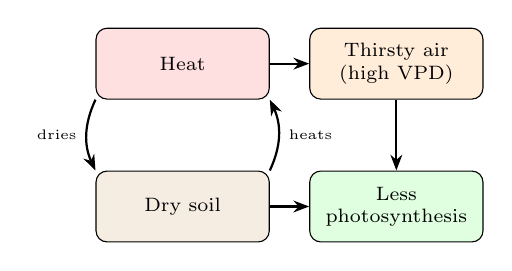
\begin{tikzpicture}[
        node distance=9mm and 5mm,
        b/.style={draw, rounded corners, align=center, font=\scriptsize,
                  minimum width=2.2cm, minimum height=0.9cm},
        a/.style={-{Stealth[length=2mm]}, thick}]
      \node[b, fill=red!12] (heat) {Heat};
      \node[b, fill=orange!15, right=of heat] (vpd) {Thirsty air\\(high VPD)};
      \node[b, fill=brown!15, below=of heat] (soil) {Dry soil};
      \node[b, fill=green!12, below=of vpd] (gpp) {Less\\photosynthesis};
      \draw[a] (heat) -- (vpd);
      \draw[a] (vpd) -- (gpp);
      \draw[a] (soil) -- (gpp);
      \draw[a] (heat.south west) to[bend right=25] node[left, font=\tiny]{dries} (soil.north west);
      \draw[a] (soil.north east) to[bend right=25] node[right, font=\tiny]{heats} (heat.south east);
    \end{tikzpicture}
  \end{columns}
\end{frame}

\begin{frame}{Why it matters}
  \begin{itemize}
    \item Plant productivity (GPP) is the base of food production and the
      land carbon sink
    \item Europe 2003: heat + drought cut productivity by $\sim$30\%
      \citep{ciais2005}
    \item Combined heat + drought hurts the carbon sink more than either alone
      \citep{vonbuttlar2018}
    \item In India, concurrent droughts and heatwaves are becoming more common
      \citep{sharma2017}
  \end{itemize}
\end{frame}

\begin{frame}{Why India?}
  \begin{columns}
    \column{0.40\linewidth}
    \begin{itemize}
      \item \textbf{Monsoon-dependent}: weak monsoon $\Rightarrow$ drought
        (2002, 2009)
      \item \textbf{Hot pre-monsoon}: extreme heat in 2010, 2022
      \item \textbf{Mostly cropland} ($\sim$60\% of grid cells)
      \item \textbf{Under-studied}: India-wide work is only just appearing
        \citep{meena2026,sen2026}
    \end{itemize}
    \column{0.60\linewidth}
    \centering
    \includegraphics[width=\linewidth,height=0.78\textheight,keepaspectratio]{\FigPath{study_area_landcover}}
  \end{columns}
\end{frame}

\begin{frame}{Problem statement}
  \textbf{Topic \#19:} Does simultaneous heat and drought produce greater
  ecosystem stress than either alone?

  \vspace{8pt}
  \textbf{Our questions (India):}
  \begin{enumerate}
    \item Are compound months worse than hot-only or dry-only months?
    \item Are they worse than the two effects \emph{added together}?
    \item Is recovery slower after compound events?
    \item Does it differ by land cover and region?
  \end{enumerate}

  \vspace{6pt}
  \small \textit{Why ``added together'' matters: if additive, compound impacts
  are predictable from single stresses; if not, they are a separate risk.}
\end{frame}

\begin{frame}{Known vs.\ open}
  \begin{columns}[T]
    \column{0.48\linewidth}
    \textbf{Known}
    \begin{itemize}
      \item Compound worse than single extremes \citep{vonbuttlar2018}
      \item India: higher \emph{probability} of vegetation drought
        \citep{meena2026}
      \item Peninsular forests: higher GPP-loss risk \citep{sen2026}
    \end{itemize}
    \column{0.5\linewidth}
    \textbf{Open}
    \begin{itemize}
      \item Is the effect on \emph{average} productivity more than additive?
      \item Does the drought definition change the answer? \citep{liang2026}
      \item Recovery: studies disagree \citep{yao2024,feng2026}
    \end{itemize}
  \end{columns}
\end{frame}

% =================================================================
\section{Our hypotheses}
% =================================================================

\begin{frame}{Our hypotheses}
  \renewcommand{\arraystretch}{1.3}
  \begin{tabular}{@{}L{0.07\linewidth}L{0.58\linewidth}L{0.3\linewidth}@{}}
    \toprule
    & \textbf{Hypothesis} & \textbf{Status} \\
    \midrule
    \textbf{H1} & Compound months have lower GPP / NDVI than single-stress months & Tested \\
    \textbf{H2} & The compound effect is \emph{more} than heat + drought added & Tested \\
    \textbf{H3} & Recovery is slower after compound events & Final evaluation \\
    \textbf{H4} & Effects differ by land cover and region & Final evaluation \\
    \bottomrule
  \end{tabular}
\end{frame}

% =================================================================
\section{Methodology}
% =================================================================

\begin{frame}{Data}
  \small
  \begin{tabular}{@{}lll@{}}
    \toprule
    \textbf{Dataset} & \textbf{Variable} & \textbf{Use} \\
    \midrule
    ERA5-Land \citep{munozsabater2021} & max temperature, soil moisture, VPD & heat \\
    SPEI \citep{vicenteserrano2010} & SPEI-3 & drought \\
    CHIRPS \citep{funk2015} & rainfall (SPI-3) & drought check \\
    MODIS \citep{running2015} & GPP & productivity \\
    MODIS \citep{didan2021} & NDVI & greenness \\
    ESA WorldCover \citep{zanaga2022} & land cover & masks, groups \\
    \bottomrule
  \end{tabular}

  \vspace{8pt}
  All of India, 0.25\textdegree{} grid, monthly; vegetation 2001--2022, climate
  1991--2024; processed in Google Earth Engine \citep{gorelick2017}.
\end{frame}

\begin{frame}{Metrics}
  \small
  \renewcommand{\arraystretch}{1.15}
  \begin{tabular}{@{}ll@{}}
    \toprule
    \textbf{GPP} & carbon taken up by plants (productivity) \\
    \textbf{NDVI} & canopy greenness \\
    \textbf{Tmax $z$} & temperature anomaly; $\ge 1$ = hot \\
    \textbf{SPEI-3} & 3-month water balance; $\le -1$ = dry \\
    \textbf{SPI-3} & rainfall-only drought index (check) \\
    \textbf{VPD} & how ``thirsty'' the air is \\
    \textbf{$z$-score} & distance from normal, in standard deviations \\
    \textbf{Amplification} & compound $-$ (heat + drought); $<0$ = synergy \\
    \bottomrule
  \end{tabular}
\end{frame}

\begin{frame}{Workflow}
  \centering
  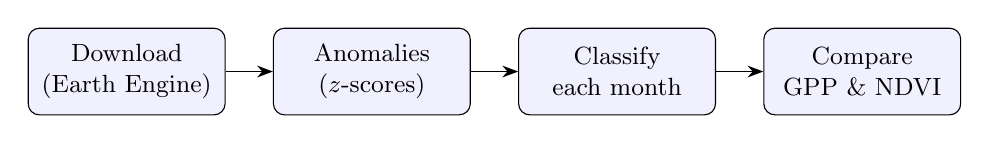
\begin{tikzpicture}[
      node distance=6mm,
      box/.style={draw, rounded corners, align=center, minimum width=2.5cm,
                  minimum height=1.1cm, font=\small, fill=blue!6},
      arr/.style={-{Stealth[length=2mm]}}]
    \node[box] (a) {Download\\(Earth Engine)};
    \node[box, right=of a] (b) {Anomalies\\($z$-scores)};
    \node[box, right=of b] (c) {Classify\\each month};
    \node[box, right=of c] (d) {Compare\\GPP \& NDVI};
    \draw[arr] (a) -- (b); \draw[arr] (b) -- (c); \draw[arr] (c) -- (d);
  \end{tikzpicture}

  \vspace{12pt}
  \begin{itemize}
    \item Anomalies remove the seasonal cycle and long-term trends
    \item Only growing-season months of vegetated Indian cells
    \item 95\% confidence intervals by resampling whole years
  \end{itemize}
\end{frame}

\begin{frame}{Four types of month}
  \begin{columns}
    \column{0.5\linewidth}
    \centering
    \renewcommand{\arraystretch}{1.4}
    \begin{tabular}{cc|c|c}
      & & \multicolumn{2}{c}{SPEI-3} \\
      & & $> -1$ & $\le -1$ \\
      \hline
      \multirow{2}{*}{Tmax $z$} & $< 1$ & Normal & Dry-only \\
      & $\ge 1$ & Hot-only & \textbf{Compound} \\
    \end{tabular}
    \column{0.48\linewidth}
    \begin{itemize}
      \item 824,598 growing-season months
      \item 7.6\% are compound
      \item Repeated with SPI-3 as a check
    \end{itemize}
  \end{columns}

  \vspace{10pt}
  \centering
  \small Amplification $= \Delta_{\text{compound}} - (\Delta_{\text{hot}} +
  \Delta_{\text{dry}})$ \quad ($<0$ synergy, $\approx 0$ additive)
\end{frame}

% =================================================================
\section{Preliminary analysis (H1, H2)}
% =================================================================

\begin{frame}{Data check}
  \centering
  \Fig{qc_jjas_anomalies}{0.72\linewidth}

  \small Known droughts (2002, 2009) and heatwaves (2010, 2022) show up clearly.
\end{frame}

\begin{frame}{Where compound months happen}
  \begin{columns}
    \column{0.5\linewidth}
    \centering
    \Fig{freq_map_compound}{\linewidth}
    \column{0.48\linewidth}
    \begin{itemize}
      \item 7.6\% of growing-season months
      \item Hotspots: northern plains, east-central India, North-East
    \end{itemize}
  \end{columns}
\end{frame}

\begin{frame}{H1: compound months are the worst}
  \centering
  \Fig{composite_gpp_z_overall}{0.47\linewidth}
  \hfill
  \Fig{composite_ndvi_z_overall}{0.47\linewidth}

  \small Compound: GPP $-0.43$, NDVI $-0.68$, significantly below both
  hot-only and dry-only.
\end{frame}

\begin{frame}{H1: why?}
  \begin{tabular}{@{}lcccc@{}}
    \toprule
    & Normal & Hot & Dry & \textbf{Compound} \\
    \midrule
    Soil moisture $z$ & $+0.29$ & $-0.75$ & $-0.38$ & $\mathbf{-1.04}$ \\
    Air dryness (VPD) $z$ & $-0.38$ & $+1.11$ & $+0.18$ & $\mathbf{+1.43}$ \\
    \bottomrule
  \end{tabular}

  \vspace{10pt}
  \begin{itemize}
    \item Compound months: driest soil \emph{and} thirstiest air
    \item Same result with the rainfall-only index (SPI-3)
    \item \textbf{H1 supported}
  \end{itemize}
\end{frame}

\begin{frame}{H2: worse than the sum?}
  \centering
  \includegraphics[width=0.9\linewidth]{\FigPath{additivity_gpp_ndvi}}

  \small Observed compound (green) is no worse than heat + drought added
  together (hatched).
\end{frame}

\begin{frame}{H2: result}
  \begin{columns}
    \column{0.46\linewidth}
    \centering
    \begin{tabular}{@{}lrr@{}}
      \toprule
      Amplification & SPEI-3 & SPI-3 \\
      \midrule
      GPP  & $+0.09$ & $-0.00$ \\
      NDVI & $+0.18$ & $+0.06$ \\
      \bottomrule
    \end{tabular}

    \vspace{4pt}
    \scriptsize ($<0$ would mean synergy)
    \column{0.52\linewidth}
    \begin{itemize}
      \item Never significantly below 0
      \item Effects roughly \textbf{add up}
      \item \textbf{H2 not supported}
    \end{itemize}
  \end{columns}
\end{frame}

\begin{frame}{H2: response surface}
  \begin{columns}
    \column{0.5\linewidth}
    \centering
    \Fig{response_surface_gpp}{\linewidth}
    \column{0.48\linewidth}
    \begin{itemize}
      \item GPP for every heat $\times$ dryness combination
      \item Dryness is the main driver
      \item Hot + dry corner is the lowest
    \end{itemize}
  \end{columns}
\end{frame}

\begin{frame}{Observations so far}
  \begin{itemize}
    \item \textbf{H1 supported}: compound months hurt vegetation most
    \item \textbf{H2 not supported}: the effect is about additive, not more
    \item Cause: dry soil + thirsty air together
    \item Drought definition (SPEI vs SPI) changes the details
    \item Caveat: MODIS GPP is partly modelled; NDVI is from the same satellite
  \end{itemize}
\end{frame}

% =================================================================
\section{Things left to do}
% =================================================================

\begin{frame}{Improving H2: regression instead of four boxes}
  \[
    \text{GPP} = a \times \text{heat} + b \times \text{dryness}
      + c \times (\text{heat} \times \text{dryness})
  \]
  \begin{itemize}
    \item Uses actual values, with no cut-offs
    \item $c < 0$ $\Rightarrow$ heat hurts more when dry (synergy)
    \item One direct test, with uncertainty
  \end{itemize}
\end{frame}

\begin{frame}{Next steps}
  \begin{columns}[T]
    \column{0.48\linewidth}
    \textbf{H3: recovery}
    \begin{itemize}
      \item Time to recover after each event
      \item Compound vs drought at equal severity
    \end{itemize}

    \vspace{6pt}
    \textbf{H4: land cover \& region}
    \begin{itemize}
      \item Forests, croplands, grasslands
      \item Peninsular vs North India
    \end{itemize}
    \column{0.5\linewidth}
    \textbf{Checks}
    \begin{itemize}
      \item Independent GPP product
      \item Stricter compound definition
      \item Other thresholds and drought indices
      \item Compare with \citet{meena2026}
      \item Case studies: 2009, 2015, 2022
    \end{itemize}
  \end{columns}
\end{frame}

\begin{frame}[allowframebreaks]{References}
  \scriptsize
  \bibliography{references}
\end{frame}

\end{document}
